%---------------------------------------------------------------------------%
%-                                                                         -%
%-                           LaTeX Template                                -%
%-                                                                         -%
%---------------------------------------------------------------------------%
%- Copyright (C) Hao XIE <oaheix@gmail.com> 
%- This is free software: you can redistribute it and/or modify it
%- under the terms of the GNU General Public License as published by
%- the Free Software Foundation, either version 3 of the License, or
%- (at your option) any later version.
%---------------------------------------------------------------------------%
%->> Document class declaration
%---------------------------------------------------------------------------%
\documentclass[singlesided,cuzhdr,UTF8]{styles/cuzthesis}%
%- Multiple optional arguments:
%- [<singlesided|doublesided|printcopy>]% set one or two sided eprint or print
%- [draftversion]% show draft version information
%- [fontset=<fandol|...>]% specify font set to replace automatic detection
%- [scheme=plain]% thesis writing of international students
%- [standard options for ctex book class: draft|paper size|font size|...]%
%---------------------------------------------------------------------------%
%->> Document settings
%---------------------------------------------------------------------------%
\usepackage[super,list,table]{styles/artratex}% document settings
%- usage: \usepackage[option1,option2,...,optionN]{artratex}
%- Multiple optional arguments:
%- [bibtex|biber]% set bibliography processor and package
%- [<numbers|super|authoryear|alpha>]% set citation and reference style
%- <numbers>: textual: Jones [1]; parenthetical: [1]
%- <super>: textual: Jones superscript [1]; parenthetical: superscript [1]
%- <authoryear>: textual: Jones (1995); parenthetical: (Jones, 1995)
%- <alpha>: textual: not available; parenthetical: [Jon95]
%- [geometry]% reconfigure page layout via geometry package
%- [lscape]% provide landscape layout environment
%- [myhdr]% enable header and footer via fancyhdr package
%- [color]% provide color support via xcolor package
%- [background]% enable page background
%- [tikz]% provide complex diagrams via tikz package
%- [table]% provide complex tables via ctable package
%- [list]% provide enhanced list environments for algorithm and coding
%- [math]% enable some extra math packages
\usepackage{styles/artracom}% user defined commands
%---------------------------------------------------------------------------%
%->> Document content
%---------------------------------------------------------------------------%
\begin{document}
%-> Initialization
%---------------------------------------------------------------------------%
%-> Initialization of some info
%---------------------------------------------------------------------------%
\confidential{}% the confidential level (omitted)
\schoollogo{0.8}{cuz_logo}% the logo of university
\title{浙江传媒学院毕业论文\LaTeX{}模板}% the Chinese title of the thesis 
\englishtitle{A \LaTeX{} Thesis Template of CUZ}% the English title of the thesis
\author{???}% the author's name
\authorid{?????????}% the author's id
\advisor{???}% the advisor's name
\advisortitle{??}% the title of the advisor
\degree{学士}% the degree (must be one of {"学士","硕士","博士"})
\major{??????}% the name of the major
\institute{?????}% the name of the institute
\graduateyear{????}% the year of graduation
%---------------------------------------------------------------------------%

%-
%-> Frontmatter: title page, declaration, abstracts, content list
%-
\plainmatter% set the page layout
%-> The title page
\maketitle%
%-> The author's declaration
\makedeclaration%
\nofootermatter% change the page layout
\begin{chineseabstract}
    {浙江传媒学院,毕业论文,\hologo{LaTeX}模板,全文的浓缩}本文是浙江传媒学院本
    科毕业论文模板cuzthesis的使用说明文档。主要内容为介绍\hologo{LaTeX}文档类
    cuzthesis的用法,以及撰写毕业论文的一些拙见。

    摘要是全文的浓缩,要涵盖文章的主要内容,一般应保证字数在300以上,须包括如下
    三点:做了什么、如何做的、做得怎样。具体而言:\textbf{第一段},可以用一句话
    概述课题背景;接着再用一两句话表明做的东西。\textbf{第二段},可以用三五句话
    描述如何做的,包括做这个东西分几步(或几个模块),每步(模块)的任务,以及相
    邻步(或相关模块)之间的关系。\textbf{最后一段},用两三句话概括作品的亮点,
    以及效果怎样,包括可能的市场反响、用户体验等等。
    
    需要注意的是,既然是全文的浓缩,就不要出现类似“本项目将要做到”或者“详情见正
    文”等此类语句,因其并非正文中应出现的说法(既然已经是正文的浓缩,再说详情见
    正文就产生了矛盾)。此外,语言上应注意言简意赅,语气上应平实无感。
\end{chineseabstract}
\begin{englishabstract}
    {Communication University of Zhejiang (CUZ), thesis, \LaTeX{} Template,
    abstraction of the whole thesis} This documentation is a helper for the
    \LaTeX{} class \texttt{cuzthesis}, which is a thesis template for the
    Communication University of Zhejiang. The main content is about how to use
    the \texttt{cuzthesis}, as well as some advices of writing thesis.

    Abstract is the abstraction of the whole thesis, which should cover the main
    aspects of the thesis, and should contain no less than 300 words, involving
    3 aspects: what is done, how to do it, and what about the result.
    Specifically, \textbf{1st paragraph}, introduce the background by 1
    sentence, and what is done by 1 or 2 sentence(s). \textbf{2nd paragraph},
    describe how to do it by 3 to 5 sentences, including how many steps
    (modules) are used, what each step (module) does, and the relationship
    between adjacent steps (related modules). \textbf{Last paragraph}, extract
    the most important features of the work and its effect by 2 or 3 sentences,
    including possible responses of markets, user experiences, etc..
	
	Note that, since it is the abstraction of the whole thesis, expressions such
	as ``this project will'' or ``readers are refered to the body of thesis for
	details'' should be avoided, for this saying should not appear in the body
	of thesis (now that this is the abstraction, a refering to the body of
	thesis generates a conflict). Besides, the language should be neat, and the
	tone should be plain and without emotions.
\end{englishabstract}
%-> The table of contents
\tableofcontents%
%-
%-> Mainmatter: the main body
%-
\mainmatter% change the page layout
%---------------------------------------------------------------------------%
%->> The main body of the thesis
%---------------------------------------------------------------------------%
\chapter{绪论}\label{chap:introduction}

\section{课题背景}\label{sec:background}

考虑到许多同学可能缺乏\LaTeX{}使用经验,cuzthesis在参考了ucasthesis模板的基础
上,将\LaTeX{}的复杂性高度封装,开放出简单的接口,以便轻易使用。同时,对用
\LaTeX{}撰写论文的一些主要难题,如制图、制表、文献索引等,进行了详细说明,并提供
了相应的代码样本,理解了上述问题后,对于初学者而言,使用此模板撰写学位论文将不存
在实质性的困难。所以,如果你是初学者,请不要直接放弃,因为同样为初学者的我,十分
明白让\LaTeX{}简单易用的重要性,而这正是cuzthesis与ucasthesis所追求和体现的。

此浙传毕业论文模板cuzthesis基于国科大莫晃锐制作的ucasthesis模板发展而来。当前
cuzthesis模板满足最新的浙江传媒学院本科毕业论文撰写要求和封面设定,兼顾主流操作
系统:Windows,Linux,macOS 和主流\LaTeX{}编译引擎:\hologo{pdfLaTeX}、
\hologo{XeLaTeX}、\hologo{LuaLaTeX},详细支持情况见表\ref{tab:support-status}。
支持中文书签、中文渲染、中文粗体显示、拷贝PDF中的文本到其他文本编辑器等特性。此
外,对模板的文档结构进行了精心设计,撰写了编译脚本提高模板的易用性和使用效率。
\begin{table}[htbp]
    \caption[编译引擎跨平台情况]{各平台下编译引擎支持情况(\checkmark:支持或部分支持;$\times$:不支持)}
    \label{tab:support-status}
    \centering
    \small% fontsize
    % \setlength{\tabcolsep}{4pt}% column separation
    % \renewcommand{\arraystretch}{1.2}%row space 
    \begin{tabular}{cccc}
        \toprule
         & \hologo{pdfLaTeX} & \hologo{XeLaTeX} & \hologo{LuaLaTeX} \\
        \midrule
        Linux & $\times$ & \checkmark\footnote{暂不完全支持,粗楷体加由粗宋体代
        替,仿宋加粗无效;但不影响本模板使用。} & \checkmark\footnote{暂不完全支
        持,粗楷体加由粗宋体代替,仿宋加粗无效;但不影响本模板使用。} \\
        macOS & ?\footnote{暂未测试……} & \checkmark & ?\footnote{暂未测试……} \\
        Windows & \checkmark\footnote{暂不完全支持,粗宋体加由黑体代替。} &
        \checkmark\footnote{暂不完全支持,粗楷体由粗宋体代替;但不影响本模板使
        用。} & \checkmark\footnote{暂不完全支持,所有中文字体均无法加粗,且编译
        时间较\hologo{XeLaTeX}慢一些。} \\
        \bottomrule
    \end{tabular}
\end{table}

cuzthesis的目标在于简化毕业论文的撰写,利用\LaTeX{}格式与内容分离的特征,模板将
格式设计好后,作者可只需关注论文内容。同时,cuzthesis有着整洁一致的代码结构和扼
要的注解,对文档的仔细阅读可为初学者提供一个学习\LaTeX{}的窗口。此外,模板的架构
十分注重通用性,事实上,与ucasthesis一样,cuzthesis不仅是浙传毕业论文模板,同
时,通过少量修改即可成为使用\LaTeX{}撰写中英文文章或书籍的通用模板,并为使用者的
个性化设定提供了接口。

\section{系统要求}\label{sec:system}

\href{https://github.com/xiehao/CUZThesis}{cuzthesis}宏包可以在目前主流的
\href{https://en.wikibooks.org/wiki/LaTeX/Introduction}{\LaTeX{}}编译系统中使
用,例如C\TeX{}套装(请勿混淆C\TeX{}套装与ctex宏包。C\TeX{}套装是集成了许多
\LaTeX{}组件的\LaTeX{}编译系统,因已停止维护,\textbf{不再建议使用}。
\href{https://ctan.org/pkg/ctex?lang=en}{ctex} 宏包如同cuzthesis,是\LaTeX{}命令
集,其维护状态活跃,并被主流的\LaTeX{}编译系统默认集成,是几乎所有\LaTeX{}中文文
档的核心架构。)、MiK\TeX{}(维护较不稳定,\textbf{不太推荐使用})、\TeX{}Live。
而文本编辑器方面则包括:Visual Studio Code(简称VS Code)、\hologo{TeX}studio、
Emacs、Vim等。推荐的
\href{https://en.wikibooks.org/wiki/LaTeX/Installation}{\LaTeX{}编译系统}和
\href{https://en.wikibooks.org/wiki/LaTeX/Installation}{\LaTeX{}文本编辑器}如表
\ref{tab:recomendations}所示。
\begin{table}[htbp]
    \caption[推荐的编译系统与编辑器]{不同平台下推荐的编译系统与编辑器}
    \label{tab:recomendations}
    \centering
    \small% fontsize
    %\setlength{\tabcolsep}{4pt}% column separation
    %\renewcommand{\arraystretch}{1.5}% row space 
    \begin{tabular}{ccc}
        \toprule
        %\multicolumn{num_of_cols_to_merge}{alignment}{contents} \\
        %\cline{i-j}% partial hline from column i to column j
        操作系统 & \LaTeX{}编译系统 & \LaTeX{}文本编辑器\\
        \midrule
        Linux &
        \href{https://www.tug.org/texlive/acquire-netinstall.html}{\TeX{}Live
        Full} & \href{https://code.visualstudio.com/download}{VS Code}、
        \href{https://www.texstudio.org/}{\hologo{TeX}studio}、Emacs、Vim\\
        MacOS & \href{https://www.tug.org/mactex/}{Mac\TeX{} Full} &
        \href{https://code.visualstudio.com/download}{VS Code}、
        \href{https://www.texstudio.org/}{\hologo{TeX}studio}、Emacs\\
        Windows &
        \href{https://www.tug.org/texlive/acquire-netinstall.html}{\TeX{}Live
        Full} & \href{https://code.visualstudio.com/download}{VS Code}、
        \href{https://www.texstudio.org/}{\hologo{TeX}studio}\\
        \bottomrule
    \end{tabular}
\end{table}

\LaTeX{}编译系统,如\TeX{}Live(Mac\TeX{}为针对macOS的\TeX{}Live),用于提供编译
环境;\LaTeX{}文本编辑器 (如VS Code) 用于编辑\TeX{}源文件。请从各软件官网下载安
装程序,勿使用不明程序源。\textbf{\LaTeX{}编译系统和\LaTeX{}编辑器分别安装成功
后,即完成了\LaTeX{}的系统配置},无需其他手动干预和配置。若系统原带有旧版的
\LaTeX{}编译系统并想安装新版,请\textbf{先卸载干净旧版再安装新版}。

\section{问题反馈}\label{sec:callback}

关于\LaTeX{}的知识性问题,请查阅
\href{https://github.com/mohuangrui/ucasthesis/wiki}{ucasthesis和\LaTeX{}知识小
站} 和 \href{https://en.wikibooks.org/wiki/LaTeX}{\LaTeX{} Wikibook}。

关于模板编译和样式设计的问题,请\textbf{先仔细阅读此说明文档,特别是“常见问题”
(章节~\ref{sec:qa})}。若问题仍无法得到解决,请\textbf{先将问题理解清楚并描述清
楚,再将问题反馈}至
\href{https://github.com/xiehao/CUZThesis/issues}{Github/cuzthesis/issues}。

欢迎大家有效地反馈模板不足之处,一起不断改进模板。希望大家向同事积极推广
\LaTeX{},一起更高效地做科研。

\section{模板下载}\label{sec:download}

\begin{center}
    \href{https://github.com/xiehao/CUZThesis}{Github/cuzthesis}:
    \url{https://github.com/xiehao/CUZThesis}。
\end{center}

\chapter{\LaTeX{}使用说明}\label{chap:guide}

为方便使用及更好地展示\LaTeX{}排版的优秀特性,ucasthesis的框架和文件体系进行了细致地处理,尽可能地对各个功能和板块进行了模块化和封装,对于初学者来说,众多的文件目录也许一开始让人觉得有些无所适从,但阅读完下面的使用说明后,会发现原来使用思路是简单而清晰的,而且,当对\LaTeX{}有一定的认识和了解后,会发现其相对Word类排版系统极具吸引力的优秀特性。所以,如果是初学者,请不要退缩,请稍加尝试和坚持,以领略到\LaTeX{}的非凡魅力,并可以通过阅读相关资料如\LaTeX{} Wikibook\citep{wikibook2014latex}来完善自己的使用知识。

\section{先试试效果}

\begin{enumerate}
    \item 安装软件:根据所用操作系统和章节~\ref{sec:system}中的信息安装\LaTeX{}编译环境。
    \item 获取模板:下载 \href{https://github.com/mohuangrui/ucasthesis}{ucasthesis} 模板并解压。ucasthesis模板不仅提供了相应的类文件,同时也提供了包括参考文献等在内的完成学位论文的一切要素,所以,下载时,推荐下载整个ucasthesis文件夹,而不是单独的文档类。
    \item 编译模板:
        \begin{enumerate}
            \item Windows:双击运行artratex.bat脚本。
            \item Linux或MacOS: {\scriptsize \verb|terminal| -> \verb|chmod +x ./artratex.sh| -> \verb|./artratex.sh xa|}
            \item 任意系统:都可使用\LaTeX{}编辑器打开Thesis.tex文件并选择xelatex编译引擎进行编译。
        \end{enumerate}
    \item 错误处理:若编译中遇到了问题,请先查看“常见问题”(章节~\ref{sec:qa})。
\end{enumerate}

编译完成即可获得本PDF说明文档。而这也完成了学习使用ucasthesis撰写论文的一半进程。什么?这就学成一半了,这么简单???,是的,就这么简单!

\section{文档目录简介}

\subsection{Thesis.tex}

Thesis.tex为主文档,其设计和规划了论文的整体框架,通过对其的阅读可以了解整个论文框架的搭建。

\subsection{编译脚本}

\begin{itemize}
    \item Windows:双击Dos脚本artratex.bat可得全编译后的PDF文档,其存在是为了帮助不了解\LaTeX{}编译过程的初学者跨过编译这第一道坎,请勿通过邮件传播和接收此脚本,以防范Dos脚本的潜在风险。
    \item Linux或MacOS:在terminal中运行
        \begin{itemize}
            \item \verb|./artratex.sh xa|:获得全编译后的PDF文档
            \item \verb|./artratex.sh x|:快速编译模式
        \end{itemize}
    \item 全编译指运行 \verb|xelatex+bibtex+xelatex+xelatex| 以正确生成所有的引用链接,如目录,参考文献及引用等。在写作过程中若无添加新的引用,则可用快速编译,即只运行一遍\LaTeX{}编译引擎以减少编译时间。
\end{itemize}

\subsection{Tmp文件夹}

运行编译脚本后,编译所生成的文档皆存于Tmp文件夹内,包括编译得到的PDF文档,其存在是为了保持工作空间的整洁,因为好的心情是很重要的。

\subsection{Style文件夹}

包含ucasthesis文档类的定义文件和配置文件,通过对它们的修改可以实现特定的模版设定。若需更新模板,一般只需用新的样式文件替换旧的即可。

\begin{enumerate}
    \item ucasthesis.cls:文档类定义文件,论文的最核心的格式即通过它来定义的。
    \item ucasthesis.cfg:文档类配置文件,设定如目录显示为“目~录”而非“目录”。
    \item artratex.sty: 常用宏包及文档设定,如参考文献样式、文献引用样式、页眉页脚设定等。这些功能具有开关选项,常只需在Thesis.tex中的如下命令中进行启用即可,一般无需修改artratex.sty本身。
        
        \path{\usepackage[options]{artratex}} 
    \item artracom.sty:自定义命令以及添加宏包的推荐放置位置。
\end{enumerate}

\subsection{Tex文件夹}

文件夹内为论文的所有实体内容,正常情况下,这也是\textbf{使用ucasthesis撰写学文论文时,主要关注和修改的一个位置,注:所有文件都必须采用UTF-8编码,否则编译后将出现乱码文本},详细分类介绍如下:

\begin{itemize}
    \item Frontpage.tex:为论文中英文封面及中英文摘要。\textbf{论文封面会根据英文学位名称如Bachelor,Master,或是Doctor自动切换为相应的格式}。
    \item Mainmatter.tex:索引需要出现的Chapter。开始写论文时,可以只索引当前章节,以快速编译查看,当论文完成后,再对所有章节进行索引即可。
    \item Chap{\_}xxx.tex:为论文主体的各个章节,可根据需要添加和撰写。
    \item Appendix.tex:为附录内容
    \item Backmatter.tex:为发表文章信息和致谢部分等。
\end{itemize}

\subsection{Img文件夹}

用于放置论文中所需要的图类文件,支持格式有:.jpg, .png, .pdf。其中,\verb|ucas_logo.pdf|为国科大校徽。不建议为各章节图片建子目录,即使图片众多,若命名规则合理,图片查询亦是十分方便。

\subsection{Biblio文件夹}

\begin{enumerate}
    \item ref.bib:参考文献信息库。
    \item gbt7714-xxx.bst:符合国标的文献样式定义文件。由 \href{https://github.com/zepinglee/gbt7714-bibtex-style}{zepinglee}  开发,并满足最新国标要求。与文献样式有关的问题,请查阅开发者所提供的文档,并建议适当追踪其更新。
\end{enumerate}

\section{数学公式、图表、参考文献等功能}

\subsection{数学公式}

比如Navier-Stokes方程,如式\eqref{eq:ns}和式\eqref{eq:ns-}所示:
\begin{equation} \label{eq:ns}
    \begin{cases}
        \frac{\partial \rho}{\partial t} + \nabla\cdot(\rho\Vector{V}) = 0 \ \mathrm{times\ font\ test}\\
        \frac{\partial (\rho\Vector{V})}{\partial t} + \nabla\cdot(\rho\Vector{V}\Vector{V}) = \nabla\cdot\Tensor{\sigma} \ \text{times font test}\\
        \frac{\partial (\rho E)}{\partial t} + \nabla\cdot(\rho E\Vector{V}) = \nabla\cdot(k\nabla T) + \nabla\cdot(\Tensor{\sigma}\cdot\Vector{V})
    \end{cases}
\end{equation}
\begin{equation} \label{eq:ns-}
    \frac{\partial }{\partial t}\int\limits_{\Omega} u \, \mathrm{d}\Omega + \int\limits_{S} \unitVector{n}\cdot(u\Vector{V}) \, \mathrm{d}S = \dot{\phi}
\end{equation}

数学公式常用命令请见 \href{https://en.wikibooks.org/wiki/LaTeX/Mathematics}{WiKibook Mathematics}。artracom.sty中对一些常用数据类型如矢量矩阵等进行了封装,这样的好处是如有一天需要修改矢量的显示形式,只需单独修改artracom.sty中的矢量定义即可实现全文档的修改。

\subsection{表格}

请见表~\ref{tab:sample}。制表的更多范例,请见 \href{https://en.wikibooks.org/wiki/LaTeX/Tables}{WiKibook Tables}。
\begin{table}[!htbp]
    % \bicaption{这是一个样表。}{This is a sample table.}
    \caption{这是一个样表。}
    \label{tab:sample}
    \centering
    \footnotesize% fontsize
    \setlength{\tabcolsep}{4pt}% column separation
    \renewcommand{\arraystretch}{1.2}%row space 
    \begin{tabular}{lcccccccc}
        \hline
        Row number & \multicolumn{8}{c}{This is a multicolumn} \\
        %\cline{2-9}% partial hline from column i to column j
        \hline
        Row 1 & $1$ & $2$ & $4$ & $5$ & $6$ & $7$ & $8$\\
        Row 2 & $1$ & $2$ & $4$ & $5$ & $6$ & $7$ & $8$\\
        Row 3 & $1$ & $2$ & $4$ & $5$ & $6$ & $7$ & $8$\\
        Row 4 & $1$ & $2$ & $4$ & $5$ & $6$ & $7$ & $8$\\
        \hline
    \end{tabular}
\end{table}

\subsection{图片插入}

论文中图片的插入通常分为单图和多图,下面分别加以介绍:

单图插入:假设插入名为\verb|tc_q_criteria|(后缀可以为.jpg、.png、.pdf,下同)的图片,其效果如图\ref{fig:tc_q_criteria}。
\begin{figure}[!htbp]
    \centering
    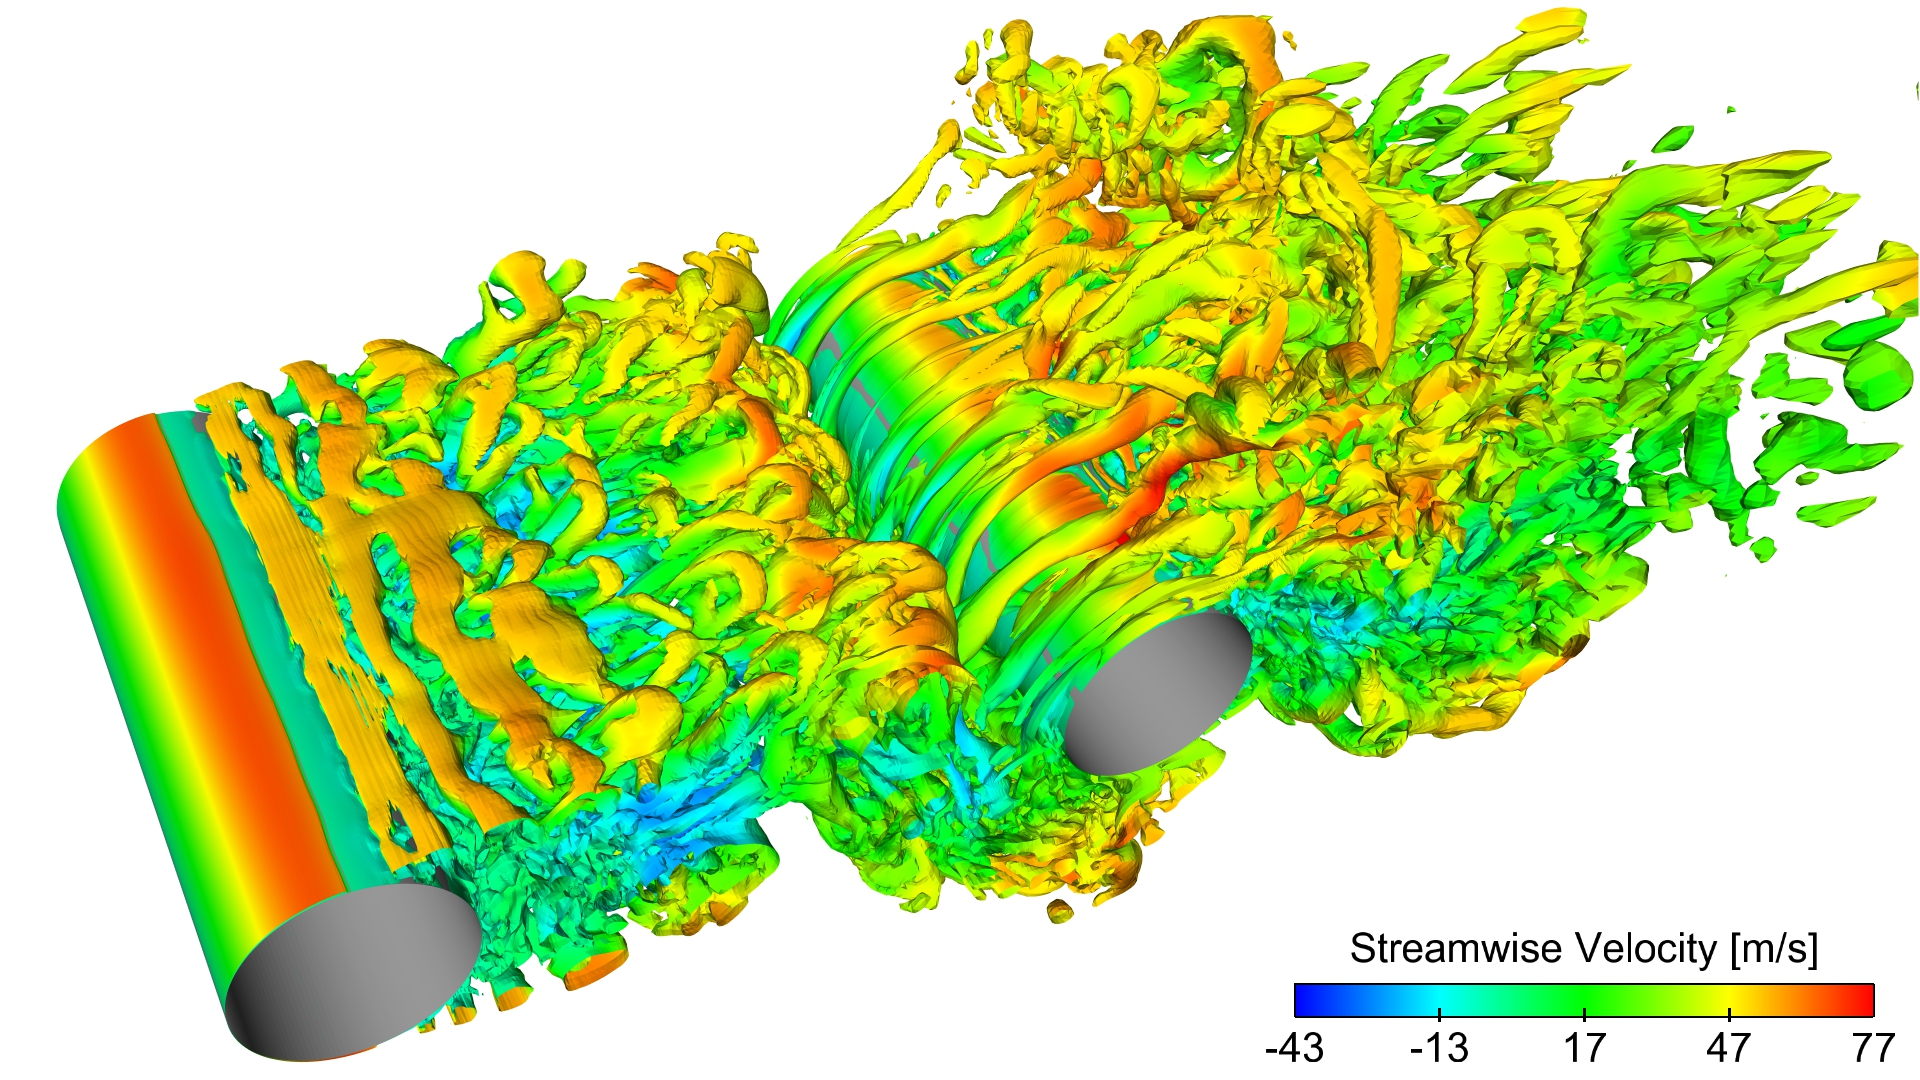
\includegraphics[width=0.40\textwidth]{tc_q_criteria}
    % \bicaption{Q判据等值面图,同时测试一下一个很长的标题,比如这真的是一个很长很长很长很长很长很长很长很长的标题。}{Isocontour of Q criteria, at the same time, this is to test a long title, for instance, this is a really very long very long very long very long very long title.}
    \caption{Q判据等值面图,同时测试一下一个很长的标题,比如这真的是一个很长很长很长很长很长很长很长很长的标题。}
    \label{fig:tc_q_criteria}
\end{figure}

如果插图的空白区域过大,以图片\verb|shock_cyn|为例,自动裁剪如图\ref{fig:shock_cyn}。
\begin{figure}[!htbp]
    \centering
    %trim option's parameter order: left bottom right top
    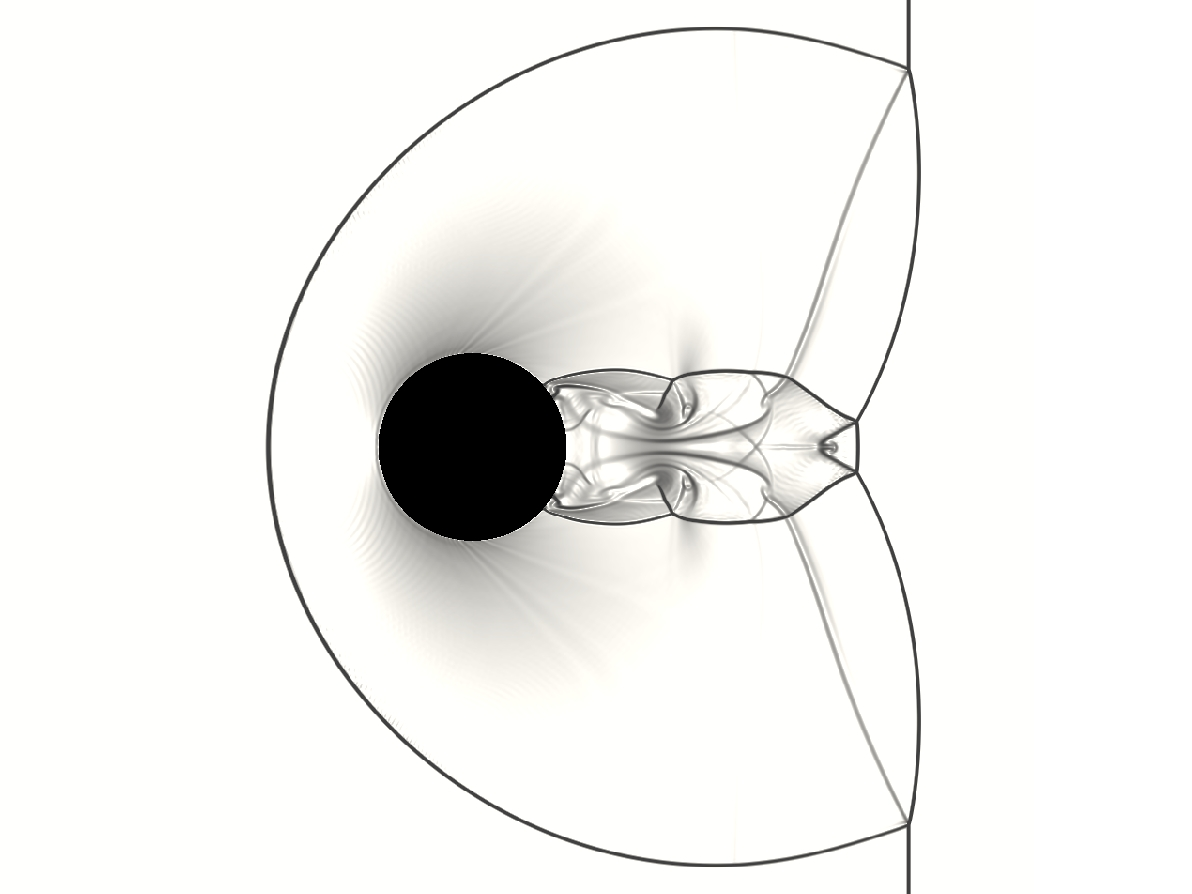
\includegraphics[trim = 30mm 0mm 30mm 0mm, clip, width=0.40\textwidth]{shock_cyn}
    % \bicaption{激波圆柱作用。}{Shock-cylinder interaction.}
    \caption{激波圆柱作用。}
    \label{fig:shock_cyn}
\end{figure}

多图的插入如图\ref{fig:oaspl},多图不应在子图中给文本子标题,只要给序号,并在主标题中进行引用说明。
\begin{figure}[!htbp]
    \centering
    \begin{subfigure}[b]{0.35\textwidth}
      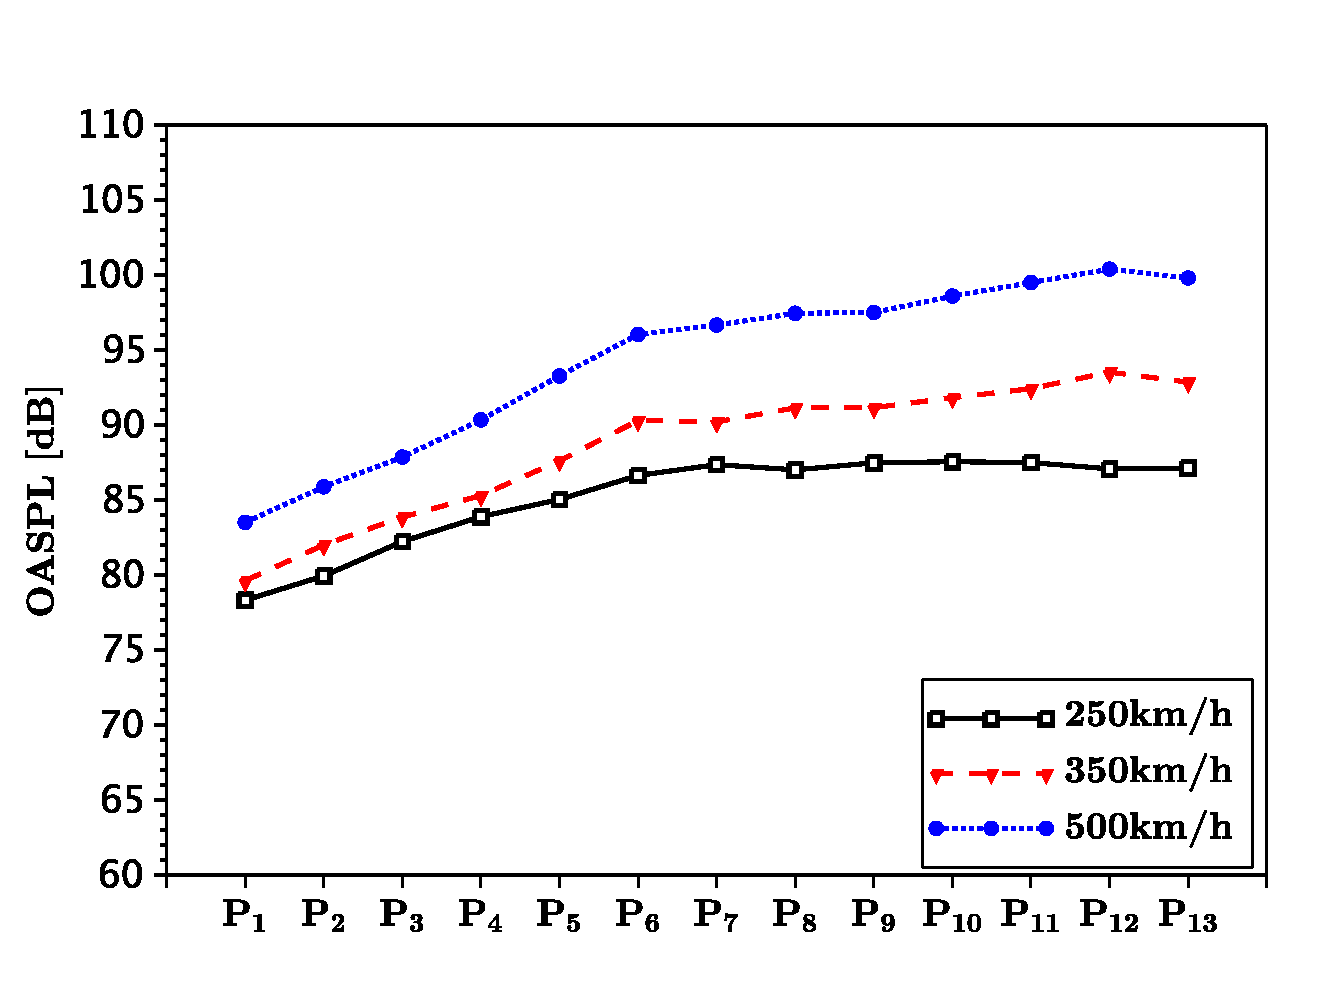
\includegraphics[width=\textwidth]{oaspl_a}
      \caption{}
      \label{fig:oaspl_a}
    \end{subfigure}%
    ~%add desired spacing
    \begin{subfigure}[b]{0.35\textwidth}
      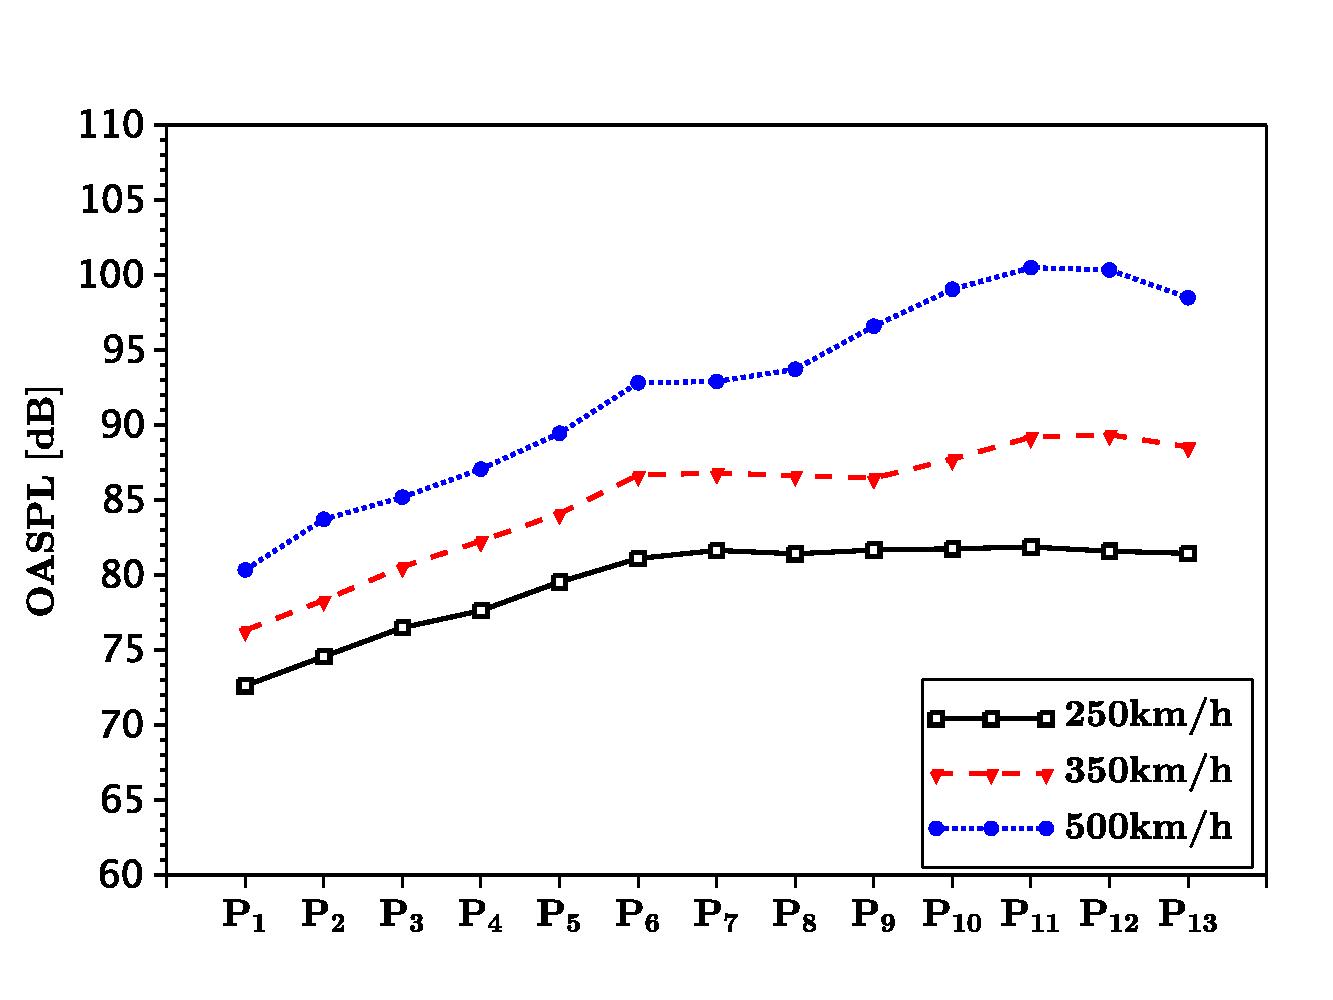
\includegraphics[width=\textwidth]{oaspl_b}
      \caption{}
      \label{fig:oaspl_b}
    \end{subfigure}
    \begin{subfigure}[b]{0.35\textwidth}
      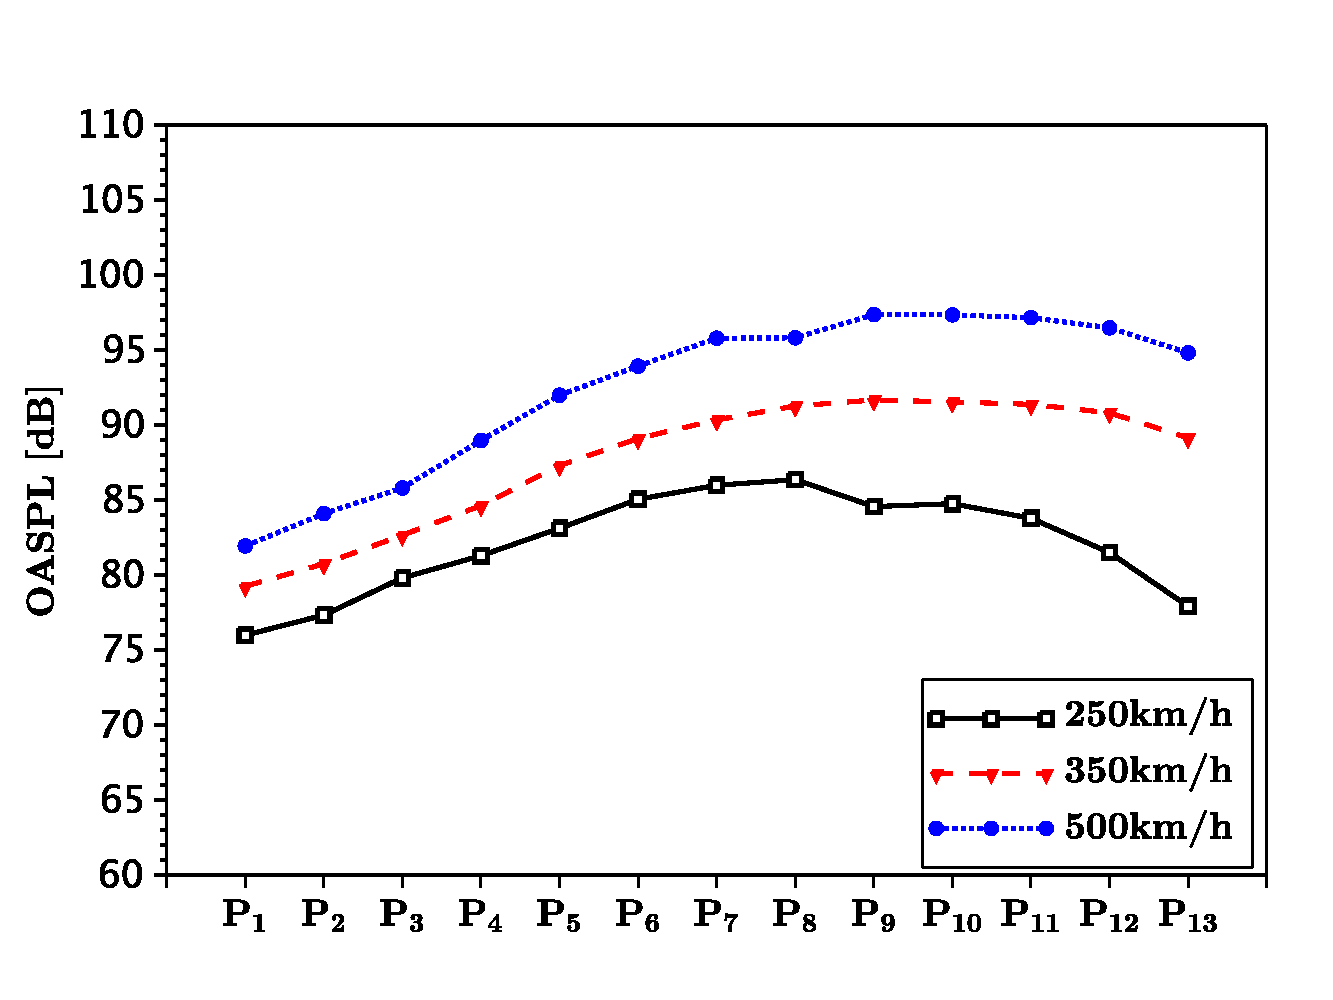
\includegraphics[width=\textwidth]{oaspl_c}
      \caption{}
      \label{fig:oaspl_c}
    \end{subfigure}%
    ~%add desired spacing
    \begin{subfigure}[b]{0.35\textwidth}
      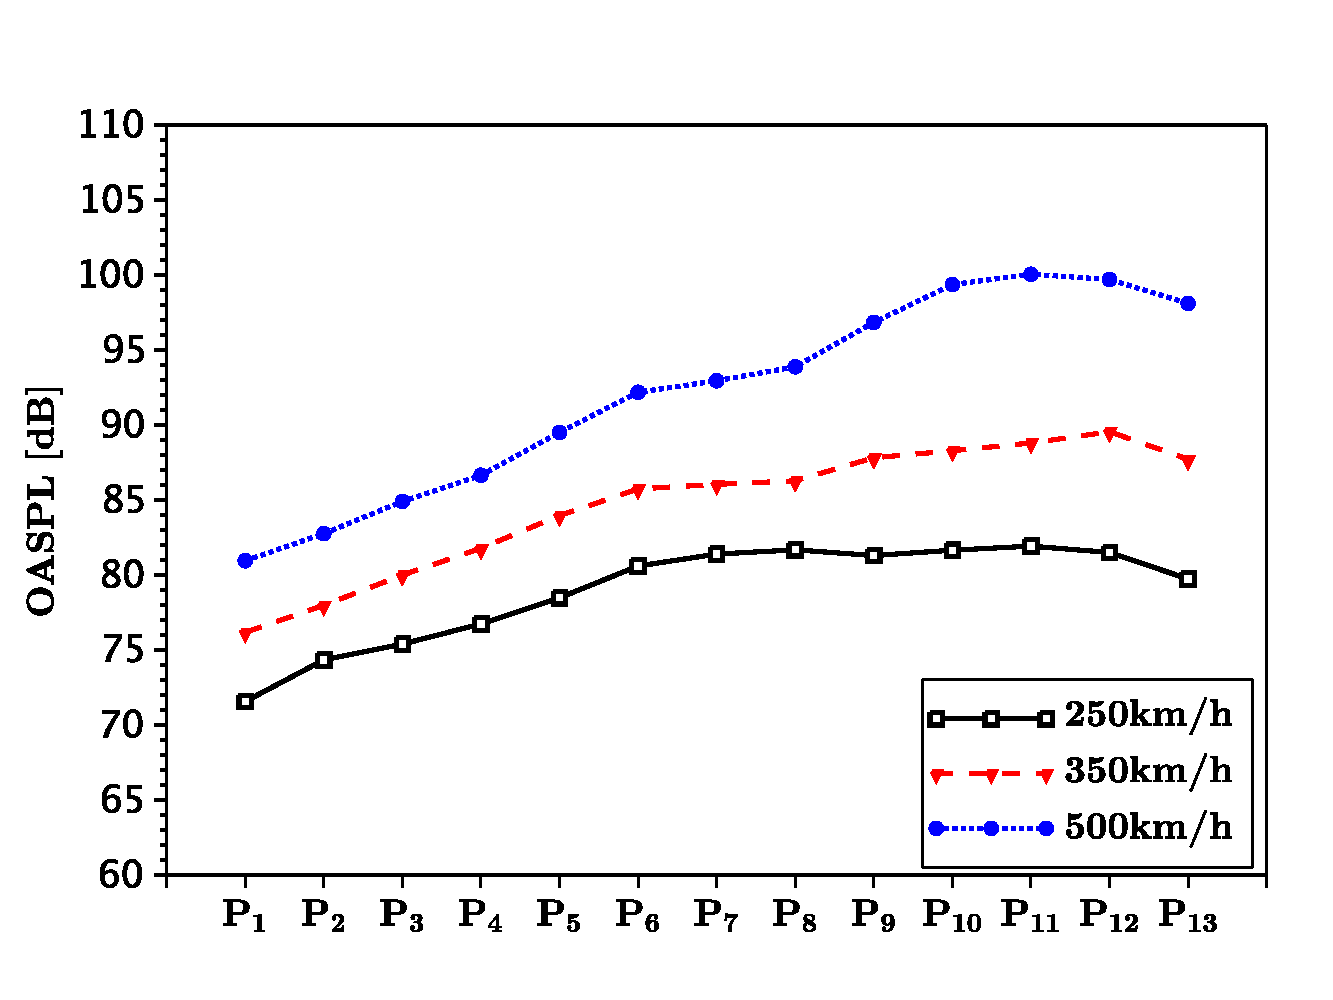
\includegraphics[width=\textwidth]{oaspl_d}
      \caption{}
      \label{fig:oaspl_d}
    \end{subfigure}
    % \bicaption{总声压级。(a) 这是子图说明信息,(b) 这是子图说明信息,(c) 这是子图说明信息,(d) 这是子图说明信息。}{OASPL.(a) This is the explanation of subfig, (b) This is the explanation of subfig, (c) This is the explanation of subfig, (d) This is the explanation of subfig.}
    \caption{总声压级。(a) 这是子图说明信息,(b) 这是子图说明信息,(c) 这是子图说明信息,(d) 这是子图说明信息。}
    \label{fig:oaspl}
\end{figure}

\subsection{算法}

如见算法~\ref{alg:euclid},详细使用方法请参见文档 \href{https://ctan.org/pkg/algorithmicx?lang=en}{algorithmicx}。

\begin{algorithm}[!htbp]
    \small
    \caption{Euclid's algorithm}\label{alg:euclid}
    \begin{algorithmic}[1]
        \Procedure{Euclid}{$a,b$}\Comment{The g.c.d. of a and b}
        \State $r\gets a\bmod b$
        \While{$r\not=0$}\Comment{We have the answer if r is 0}
        \State $a\gets b$
        \State $b\gets r$
        \State $r\gets a\bmod b$
        \EndWhile\label{euclidendwhile}
        \State \textbf{return} $b$\Comment{The gcd is b}
        \EndProcedure
    \end{algorithmic}
\end{algorithm}

\subsection{参考文献引用}

参考文献引用过程以实例进行介绍,假设需要引用名为"Document Preparation System"的文献,步骤如下:

1)使用Google Scholar搜索Document Preparation System,在目标条目下点击Cite,展开后选择Import into BibTeX打开此文章的BibTeX索引信息,将它们copy添加到ref.bib文件中(此文件位于Biblio文件夹下)。

2)索引第一行 \verb|@article{lamport1986document,|中 \verb|lamport1986document| 即为此文献的label (\textbf{中文文献也必须使用英文label},一般遵照:姓氏拼音+年份+标题第一字拼音的格式),想要在论文中索引此文献,有两种索引类型:

文本类型:\verb|\citet{lamport1986document}|。正如此处所示 \citet{lamport1986document}; 

括号类型:\verb|\citep{lamport1986document}|。正如此处所示 \citep{lamport1986document}。

\textbf{多文献索引用英文逗号隔开}:

\verb|\citep{lamport1986document, chu2004tushu, chen2005zhulu}|。正如此处所示 \citep{lamport1986document, chu2004tushu, chen2005zhulu}

更多例子如:

\citet{walls2013drought}根据...的研究,首次提出...。其中关于...\citep{walls2013drought},是当前中国...得到迅速发展的研究领域\citep{chen1980zhongguo}。引用同一著者在同一年份出版的多篇文献时,在出版年份之后用
英文小写字母区别,如:\citep{yuan2012lana, yuan2012lanb, yuan2012lanc}。同一处引用多篇文献时,按出版年份由近及远依次标注,中间用
分号分开。例如\citep{chen1980zhongguo, stamerjohanns2009mathml, hls2012jinji, niu2013zonghe}。

使用著者-出版年制(authoryear)式参考文献样式时,中文文献必须在BibTeX索引信息的 \textbf{key} 域(请参考ref.bib文件)填写作者姓名的拼音,才能使得文献列表按照拼音排序。参考文献表中的条目(不排序号),先按语种分类排列,语种顺 序是:中文、日文、英文、俄文、其他文种。然后,中文按汉语拼音字母顺序排列,日文按第一著者的姓氏笔画排序,西文和 俄文按第一著者姓氏首字母顺序排列。如中\citep{niu2013zonghe}、日\citep{Bohan1928}、英\citep{stamerjohanns2009mathml}、俄\citep{Dubrovin1906}。

如此,即完成了文献的索引,请查看下本文档的参考文献一章,看看是不是就是这么简单呢?是的,就是这么简单!

不同文献样式和引用样式,如著者-出版年制(authoryear)、顺序编码制(numbers)、上标顺序编码制(super)可在Thesis.tex中对artratex.sty调用实现,如:
\begin{itemize}
    \footnotesize
    \item \verb+\usepackage[numbers]{artratex}+ $\%$ 文本: Jones [1]; 括号: [1]
    \item \verb+\usepackage[super]{artratex}+ $\%$ 文本: Jones 上标[1]; 括号: 上标[1]
    \item \verb+\usepackage[authoryear]{artratex}+ $\%$ 文本: Jones (1995); 括号: (Jones, 1995)
    \item \verb+\usepackage[alpha]{artratex}+ $\%$ 文本: 不可用; 括号: [Jon95]
\end{itemize}

当前文档的默认参考文献样式为\textbf{authoryear}。若在上标(\textbf{super})模式下,希望在特定位置将上标改为嵌入式标,可使用

文本类型:\verb|\citetns{lamport1986document,chen2005zhulu}|。

正如此处所示\citetns{lamport1986document,chen2005zhulu}

括号类型:\verb|\citepns{lamport1986document,chen2005zhulu}|。

正如此处所示\citepns{lamport1986document,chen2005zhulu}

参考文献索引更为详细的信息,请见 \href{https://github.com/zepinglee/gbt7714-bibtex-style}{zepinglee} 和 \href{https://en.wikibooks.org/wiki/LaTeX/Bibliography_Management}{WiKibook Bibliography}。

\nocite{*}

\section{常见使用问题}\label{sec:qa}

\begin{enumerate}
    \item 模板每次发布前,都已在Windows,Linux,MacOS系统上测试通过。下载模板后,若编译出现错误,则请见 \href{https://github.com/mohuangrui/ucasthesis/wiki}{ucasthesis和\LaTeX{}知识小站} 的 \href{https://github.com/mohuangrui/ucasthesis/wiki/%E7%BC%96%E8%AF%91%E6%8C%87%E5%8D%97}{编译指南}。

    \item 模板文档的编码为UTF-8编码。所有文件都必须采用UTF-8编码,否则编译后生成的文档将出现乱码文本。若出现文本编辑器无法打开文档或打开文档乱码的问题,请检查编辑器对UTF-8编码的支持。如果使用WinEdt作为文本编辑器(\textbf{不推荐使用}),应在其Options -> Preferences -> wrapping选项卡下将两种Wrapping Modes中的内容:
        
        TeX;HTML;ANSI;ASCII|DTX...
        
        修改为:TeX;\textbf{UTF-8|ACP;}HTML;ANSI;ASCII|DTX...
        
        同时,取消Options -> Preferences -> Unicode中的Enable ANSI Format。

    \item 推荐选择xelatex或lualatex编译引擎编译中文文档。编译脚本的默认设定为xelatex编译引擎。你也可以选择不使用脚本编译,如直接使用 \LaTeX{}文本编辑器编译。注:\LaTeX{}文本编辑器编译的默认设定为pdflatex编译引擎,若选择xelatex或lualatex编译引擎,请进入下拉菜单选择。为正确生成引用链接,需要进行全编译。

    \item Texmaker使用简介
        \begin{enumerate}
            \footnotesize
            \item 使用 Texmaker “打开 (Open)” Thesis.tex。
            \item 菜单 “选项 (Options)” -> “设置当前文档为主文档 (Define as Master Document)”
            \item 菜单 “自定义 (User)” -> “自定义命令 (User Commands)” -> “编辑自定义命令 (Edit User Commands)” -> 左侧选择 “command 1”,右侧 “菜单项 (Menu Item)” 填入 Auto Build -> 点击下方“向导 (Wizard)” -> “添加 (Add)”: xelatex + bibtex + xelatex + xelatex + pdf viewer -> 点击“完成 (OK)”
            \item 使用 Auto Build 编译带有未生成引用链接的源文件,可以仅使用 xelatex 编译带有已经正确生成引用链接的源文件。
            \item 编译完成,“查看(View)” PDF,在PDF中 “ctrl+click” 可链接到相对应的源文件。
        \end{enumerate}
    
    \item 模版的设计可能地考虑了适应性。致谢等所有条目都是通过最为通用的

        \verb+\chapter{item name}+  and \verb+\section*{item name}+

        来显式实现的 (请观察Backmatter.tex),从而可以随意添加,放置,和修改,如同一般章节。对于图表目录名称则可在ucasthesis.cfg中进行修改。

    \item 设置文档样式: 在artratex.sty中搜索关键字定位相应命令,然后修改
        \begin{enumerate}
            \item 正文行距:启用和设置 \verb|\linespread{1.5}|,默认1.5倍行距。
            \item 参考文献行距:修改 \verb|\setlength{\bibsep}{0.0ex}|
            \item 目录显示级数:修改 \verb|\setcounter{tocdepth}{2}|
            \item 文档超链接的颜色及其显示:修改 \verb|\hypersetup|
        \end{enumerate}

    \item 文档内字体切换方法:
        \begin{itemize}
            \item 宋体:国科大论文模板ucasthesis 或 \textrm{国科大论文模板ucasthesis}
            \item 粗宋体:{\bfseries 国科大论文模板ucasthesis} 或 \textbf{国科大论文模板ucasthesis}
            \item 黑体:{\sffamily 国科大论文模板ucasthesis} 或 \textsf{国科大论文模板ucasthesis}
            \item 粗黑体:{\bfseries\sffamily 国科大论文模板ucasthesis} 或 \textsf{\bfseries 国科大论文模板ucasthesis}
            \item 仿宋:{\ttfamily 国科大论文模板ucasthesis} 或 \texttt{国科大论文模板ucasthesis}
            \item 粗仿宋:{\bfseries\ttfamily 国科大论文模板ucasthesis} 或 \texttt{\bfseries 国科大论文模板ucasthesis}
            \item 楷体:{\itshape 国科大论文模板ucasthesis} 或 \textit{国科大论文模板ucasthesis}
            \item 粗楷体:{\bfseries\itshape 国科大论文模板ucasthesis} 或 \textit{\bfseries 国科大论文模板ucasthesis}
        \end{itemize}

    \item 封面下划线上的文本不居中下划线,这是因为下划线前面还有字头,导致文本只能在页面居中和在下划线上居中二选一。当前封面采取页面居中。如需要调整文本在下划线上的位置,可用 \verb|\hspace{+/- n.0em}| 命令来插入或删除 n 个空格,进行手动调整,比如

        \verb|\advisor{\hspace{+3.0em} xxx~研究员~xxx单位}|
                
    有时下划线看上去粗细不一致,这是显示的问题,打印正常。
\end{enumerate}



%---------------------------------------------------------------------------%
%
%-
%-> Backmatter: acknowledgement, references, appendices (if any)
%-
%-> The acknowledgement
\begin{acknowledgement}
    感激casthesis作者吴凌云学长,gbt7714-bibtex-style
    开发者zepinglee,和ctex众多开发者们。若没有他们的辛勤付出和非凡工作,\LaTeX{}菜鸟的我是无法完成此国科大学位论文\LaTeX{}模板ucasthesis的。在\LaTeX{}中的一点一滴的成长源于开源社区的众多优秀资料和教程,在此对所有\LaTeX{}社区的贡献者表示感谢!
    
    ucasthesis国科大学位论文\LaTeX{}模板的最终成型离不开以霍明虹老师和丁云云老师为代表的国科大学位办公室老师们制定的官方指导文件和众多ucasthesis用户的热心测试和耐心反馈,在此对他们的认真付出表示感谢。特别对国科大的赵永明同学的众多有效反馈意见和建议表示感谢,对国科大本科部的陆晴老师和本科部学位办的丁云云老师的细致审核和建议表示感谢。谢谢大家的共同努力和支持,让ucasthesis为国科大学子使用\LaTeX{}撰写学位论文提供便利和高效这一目标成为可能。
\end{acknowledgement}%
%-> The references
\intotoc{\bibname}% add link to contents table and bookmark
\bibliography{bibliography/references}%
%-> The appendices (if any)
\appendix% change the page layout
% \chapter{中国科学院大学学位论文撰写要求}
\begin{appendices}

学位论文是研究生科研工作成果的集中体现,是评判学位申请者学术水平、授予其学位的主要依据,是科研领域重要的文献资料。根据《科学技术报告、学位论文和学术论文的编写格式》(GB/T 7713-1987)、《学位论文编写规则》(GB/T 7713.1-2006)和《文后参考文献著录规则》(GB7714—87)等国家有关标准,结合中国科学院大学(以下简称“国科大”)的实际情况,特制订本规定。

\section*{论文无附录者无需附录部分}

\section*{测试公式编号} \label{sec:testmath}

\begin{equation} \label{eq:appedns}
    \begin{cases}
        \frac{\partial \rho}{\partial t} + \nabla\cdot(\rho\Vector{V}) = 0 \ \mathrm{times\ font\ test}\\
        \frac{\partial (\rho\Vector{V})}{\partial t} + \nabla\cdot(\rho\Vector{V}\Vector{V}) = \nabla\cdot\Tensor{\sigma} \ \text{times font test}\\
        \frac{\partial (\rho E)}{\partial t} + \nabla\cdot(\rho E\Vector{V}) = \nabla\cdot(k\nabla T) + \nabla\cdot(\Tensor{\sigma}\cdot\Vector{V})
    \end{cases}
\end{equation}
\begin{equation}
    \frac{\partial }{\partial t}\int\limits_{\Omega} u \, \mathrm{d}\Omega + \int\limits_{S} \unitVector{n}\cdot(u\Vector{V}) \, \mathrm{d}S = \dot{\phi}
\end{equation}

\section*{测试生僻字}

霜蟾盥薇曜灵霜颸妙鬘虚霩淩澌菀枯菡萏泬寥窅冥毰毸濩落霅霅便嬛岧峣瀺灂姽婳愔嫕飒纚棽俪緸冤莩甲摛藻卮言倥侗椒觞期颐夜阑彬蔚倥偬澄廓簪缨陟遐迤逦缥缃鹣鲽憯懔闺闼璀错媕婀噌吰澒洞阛闠覼缕玓瓑逡巡諓諓琭琭瀌瀌踽踽叆叇氤氲瓠犀流眄蹀躞赟嬛茕頔璎珞螓首蘅皋惏悷缱绻昶皴皱颟顸愀然菡萏卑陬纯懿犇麤掱暒 墌墍墎墏墐墒墒墓墔墕墖墘墖墚墛坠墝增墠墡墢墣墤墥墦墧墨墩墪樽墬墭堕墯墰墱墲坟墴墵垯墷墸墹墺墙墼墽垦墿壀壁壂壃壄壅壆坛壈壉壊垱壌壍埙壏壐壑壒压壔壕壖壗垒圹垆壛壜壝垄壠壡坜壣壤壥壦壧壨坝塆圭嫶嫷嫸嫹嫺娴嫼嫽嫾婳妫嬁嬂嬃嬄嬅嬆嬇娆嬉嬊娇嬍嬎嬏嬐嬑嬒嬓嬔嬕嬖嬗嬘嫱嬚嬛嬜嬞嬟嬠嫒嬢嬣嬥嬦嬧嬨嬩嫔嬫嬬奶嬬嬮嬯婴嬱嬲嬳嬴嬵嬶嬷婶嬹嬺嬻嬼嬽嬾嬿孀孁孂娘孄孅孆孇孆孈孉孊娈孋孊孍孎孏嫫婿媚嵭嵮嵯嵰嵱嵲嵳嵴嵵嵶嵷嵸嵹嵺嵻嵼嵽嵾嵿嶀嵝嶂嶃崭嶅嶆岖嶈嶉嶊嶋嶌嶍嶎嶏嶐嶑嶒嶓嵚嶕嶖嶘嶙嶚嶛嶜嶝嶞嶟峤嶡峣嶣嶤嶥嶦峄峃嶩嶪嶫嶬嶭崄嶯嶰嶱嶲嶳岙嶵嶶嶷嵘嶹岭嶻屿岳帋巀巁巂巃巄巅巆巇巈巉巊岿巌巍巎巏巐巑峦巓巅巕岩巗巘巙巚帠帡帢帣帤帨帩帪帬帯帰帱帲帴帵帷帹帺帻帼帽帾帿幁幂帏幄幅幆幇幈幉幊幋幌幍幎幏幐幑幒幓幖幙幚幛幜幝幞帜幠幡幢幤幥幦幧幨幩幪幭幮幯幰幱庍庎庑庖庘庛庝庠庡庢庣庤庥庨庩庪庬庮庯庰庱庲庳庴庵庹庺庻庼庽庿廀厕廃厩廅廆廇廋廌廍庼廏廐廑廒廔廕廖廗廘廙廛廜廞庑廤廥廦廧廨廭廮廯廰痈廲廵廸廹廻廼廽廿弁弅弆弇弉弖弙弚弜弝弞弡弢弣弤弨弩弪弫弬弭弮弰弲弪弴弶弸弻弼弽弿彖彗彘彚彛彜彝彞彟彴彵彶彷彸役彺彻彽彾佛徂徃徆徇徉后徍徎徏径徒従徔徕徖徙徚徛徜徝从徟徕御徢徣徤徥徦徧徨复循徫旁徭微徯徰徱徲徳徴徵徶德徸彻徺忁忂惔愔忇忈忉忔忕忖忚忛応忝忞忟忪挣挦挧挨挩挪挫挬挭挮挰掇授掉掊掋掍掎掐掑排掓掔掕挜掚挂掜掝掞掟掠采探掣掤掦措掫掬掭掮掯掰掱掲掳掴掵掶掸掹掺掻掼掽掾掿拣揁揂揃揅揄揆揇揈揉揊揋揌揍揎揑揓揔揕揖揗揘揙揤揥揦揧揨揫捂揰揱揲揳援揵揶揷揸揻揼揾揿搀搁搂搃搄搅搇搈搉搊搋搌搎搏搐搑搒摓摔摕摖摗摙摚摛掼摝摞摠摡斫斩斮斱斲斳斴斵斶斸旪旫旮旯晒晓晔晕晖晗晘晙晛晜晞晟晠晡晰晣晤晥晦晧晪晫晬晭晰晱晲晳晴晵晷晸晹晻晼晽晾晿暀暁暂暃暄暅暆暇晕晖暊暋暌暍暎暏暐暑暒暓暔暕暖暗旸暙暚暛暜暝暞暟暠暡暣暤暥暦暧暨暩暪暬暭暮暯暰昵暲暳暴暵暶暷暸暹暺暻暼暽暾暿曀曁曂曃晔曅曈曊曋曌曍曎曏曐曑曒曓曔曕曗曘曙曚曛曜曝曞曟旷曡曢曣曤曥曦曧昽曩曪曫晒曭曮曯椗椘椙椚椛検椝椞椟椠椡椢椣椤椥椦椧椨椩椪椫椬椭椮椯椰椱椲椳椴椵椶椷椸椹椺椻椼椽椾椿楀楁楂楃楅楆楇楈楉杨楋楌楍榴榵榶榷榸榹榺榻榼榽榾桤槀槁槂盘槄槅槆槇槈槉槊构槌枪槎槏槐槑槒杠槔槕槖槗滙滛滜滝滞滟滠滢滣滦滧滪滫沪滭滮滰滱渗滳滵滶滹滺浐滼滽漀漃漄漅漈漉溇漋漌漍漎漐漑澙熹漗漘漙沤漛漜漝漞漟漡漤漥漦漧漨漪渍漭漮漯漰漱漳漴溆漶漷漹漺漻漼漽漾浆潀颍潂潃潄潅潆潇潈潉潊潋潌潍潎潏潐潒潓洁潕潖潗潘沩潚潜潝潞潟潠潡潢潣润潥潦潧潨潩潪潫潬潭浔溃潱潲潳潴潵潶滗潸潹潺潻潼潽潾涠澁澄澃澅浇涝澈澉澊澋澌澍澎澏湃澐澑澒澓澔澕澖涧澘澙澚澛澜澝澞澟渑澢澣泽浍澯澰淀澲澳澴澵澶澷澸潇潆瀡瀢瀣瀤瀥潴泷濑瀩瀪瀫瀬瀭瀮瀯弥瀱潋瀳瀴瀵瀶瀷瀸瀹瀺瀻瀼瀽澜瀿灀灁瀺灂沣滠灅灆灇灈灉灊灋灌灍灎灏灐洒灒灓漓灖灗滩灙灚灛灜灏灞灟灠灡灢湾滦灥灦灧灨灪燝燞燠燡燢燣燤燥灿燧燨燩燪燫燮燯燰燱燲燳烩燵燵燸燹燺薰燽焘燿爀爁爂爃爄爅爇爈爉爊爋爌烁爎爏爑爒爓爔爕爖爗爘爙爚烂爜爝爞爟爠爡爢爣爤爥爦爧爨爩猽猾獀犸獂獆獇獈獉獊獋獌獍獏獐獑獒獓獔獕獖獗獘獙獚獛獜獝獞獟獠獡獢獣獤獥獦獧獩狯猃獬獭狝獯狞獱獳獴獶獹獽獾獿猡玁玂玃。

\end{appendices}%
\end{document}
%---------------------------------------------------------------------------%

